\chapter{Diagramme de contexte}

Le diagramme de contexte permet de simplifier et visualiser les objectifs du projet comme étant un système qui convertit des entrées en sorties.
En effet, en faisant abstraction du robot on obtient un système causal qui interprète des signaux externes pour établir des actions précises.

\begin{figure}[h]
  \centering
  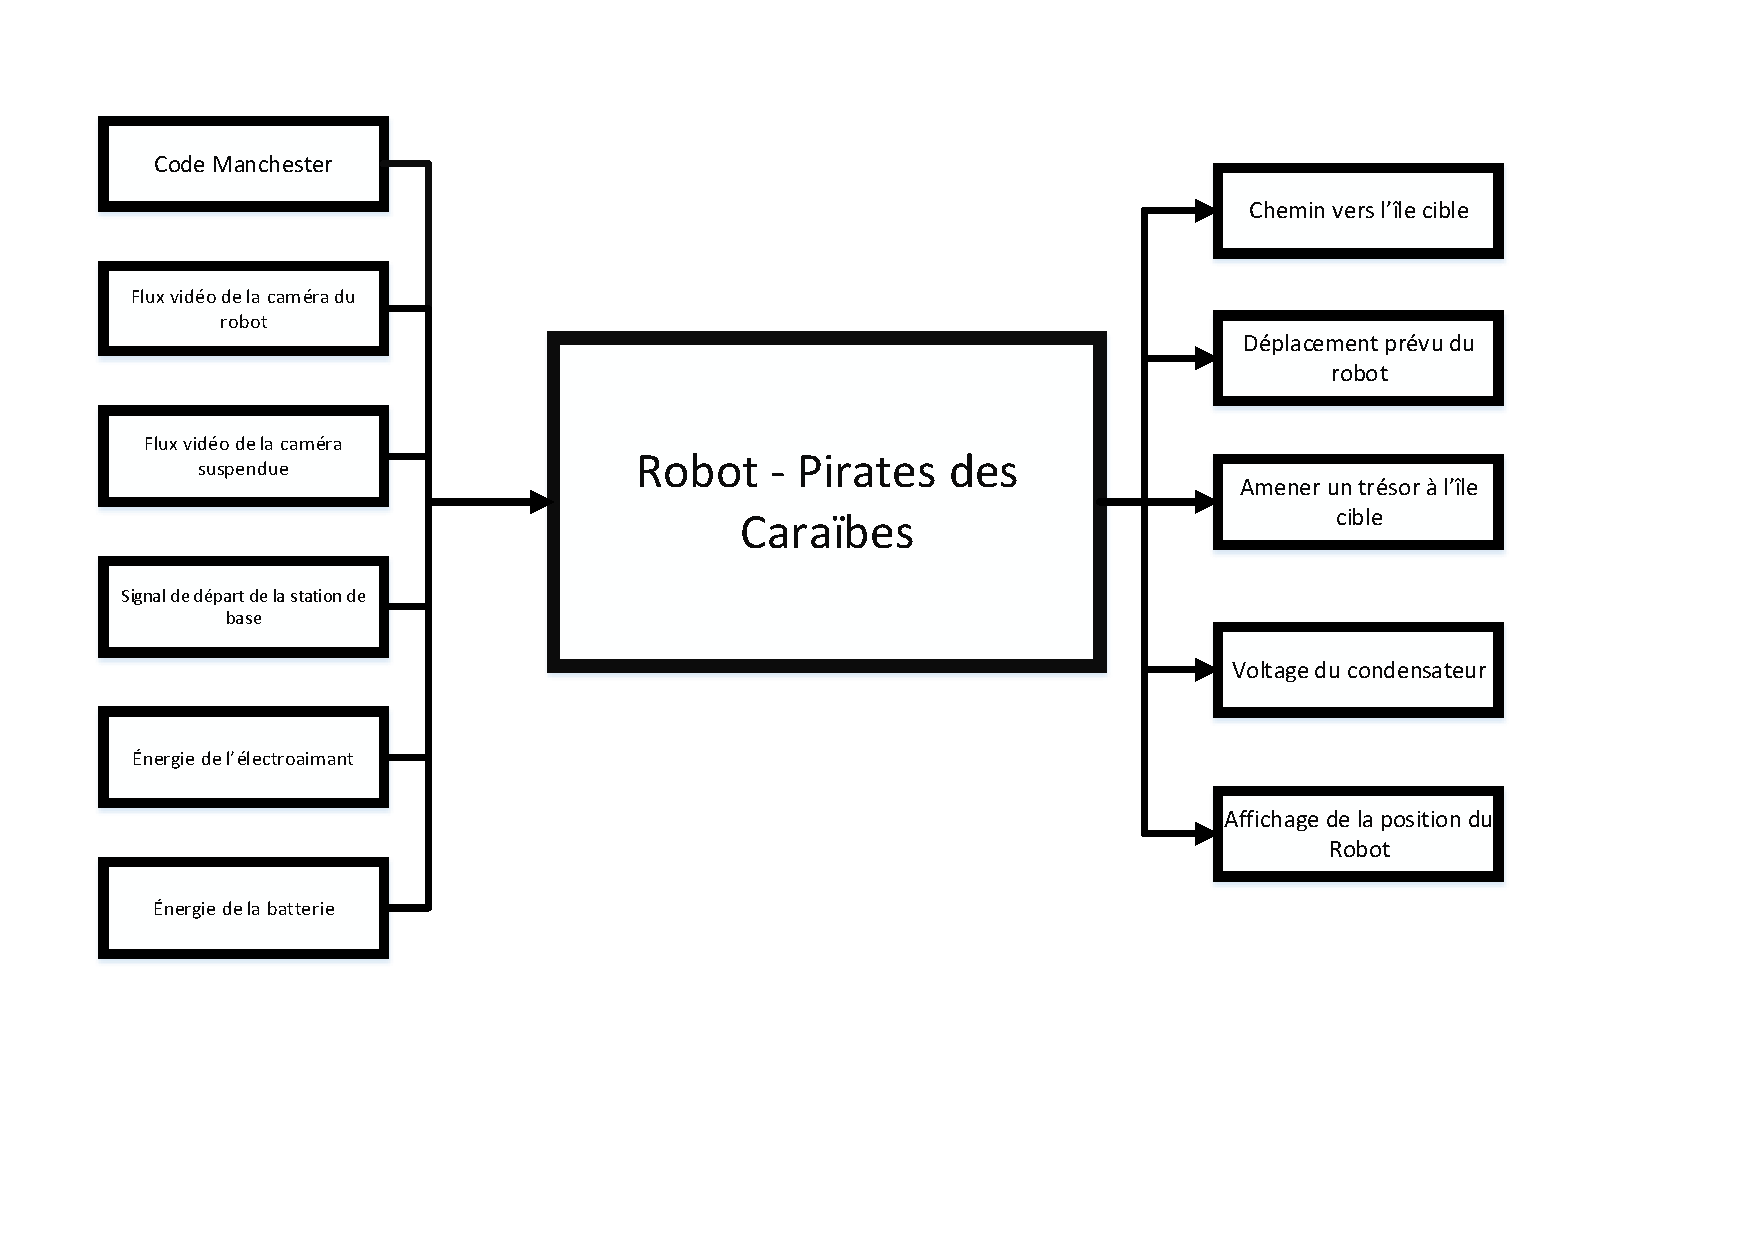
\includegraphics[scale=0.6, trim = 5mm 15mm 10mm 5mm, clip]{resources/diag_cont.pdf}
  \caption{DPF}
\end{figure}
